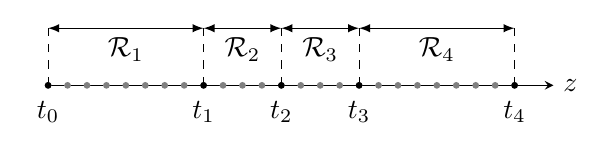
\begin{tikzpicture}
	\begin{axis}[width=8cm,height=4cm,xmin=0,xmax=6.5,xlabel=$z$,axis x line=middle,axis y line=none,xtick={0,2,3,4,6},xticklabels={$t_0$,$t_1$,$t_2$,$t_3$,$t_4$},xtick style={draw=none},every axis x label/.style={at=(current axis.right of origin),anchor=west},domain=0:6]
		\addplot[mark=*,mark size=1pt,only marks,color=gray] {0};
		\addplot[mark=*,mark size=1pt,only marks,color=black] coordinates{(0,0) (2,0) (3,0) (4,0) (6,0)};
		\draw[color=black,dashed] (0,0) -- (0,0.6);
		\draw[color=black,dashed] (2,0) -- (2,0.6);
		\draw[color=black,dashed] (3,0) -- (3,0.6);
		\draw[color=black,dashed] (4,0) -- (4,0.6);
		\draw[color=black,dashed] (6,0) -- (6,0.6);
		\draw[latex-latex] (0,0.6) -- (2,0.6) node[below,midway]{$\mathcal{R}_1$};
		\draw[latex-latex] (2,0.6) -- (3,0.6) node[below,midway]{$\mathcal{R}_2$};
		\draw[latex-latex] (3,0.6) -- (4,0.6) node[below,midway]{$\mathcal{R}_3$};
		\draw[latex-latex] (4,0.6) -- (6,0.6) node[below,midway]{$\mathcal{R}_4$};
	\end{axis}
\end{tikzpicture}
